\documentclass[12pt]{article}
\usepackage[utf8]{inputenc}
\usepackage[T1]{fontenc}
\usepackage{amsmath}
\usepackage{amsfonts}
\usepackage{amssymb}
\usepackage[version=4]{mhchem}
\usepackage{stmaryrd}
\usepackage{graphicx}
\usepackage[export]{adjustbox}
\usepackage{tikz}
\usepackage{hyperref}

\usepackage{listings} % Required for insertion of code
\usepackage{xcolor} % Required for custom colors

% Define custom colors
\definecolor{codegreen}{rgb}{0,0.6,0}
\definecolor{codegray}{rgb}{0.5,0.5,0.5}
\definecolor{codepurple}{rgb}{0.58,0,0.82}
\definecolor{backcolour}{rgb}{0.95,0.95,0.92}

% Setup the style for code listings
\lstdefinestyle{mystyle}{
    backgroundcolor=\color{backcolour},   
    commentstyle=\color{codegreen},
    keywordstyle=\color{magenta},
    numberstyle=\tiny\color{codegray},
    stringstyle=\color{codepurple},
    basicstyle=\ttfamily\footnotesize,
    breakatwhitespace=false,         
    breaklines=true,                 
    captionpos=b,                    
    keepspaces=true,                 
    numbers=left,                    
    numbersep=5pt,                  
    showspaces=false,                
    showstringspaces=false,
    showtabs=false,                  
    tabsize=2
}

% Activate the style
\lstset{style=mystyle}

\graphicspath{ {./images/} }

\title{Problem 3. Photon Echo }

\author{}
\date{}


\begin{document}
\maketitle
The following problems will help you understand the effects of quantum optics on the different types of optical spectroscopy we all use in the lab. For all plots, you can choose the value of $\omega t$, etc for easiest graphing. Normalize your curves for easy comparison in Problem 1 and Problem 2, but not Problem 3.

\section{Linear Spectroscopy}

Linear spectroscopy is good for understanding the transition energy, but little information can be gained on lifetimes. To see this, let's look at a generalized absorption cross section:

$\sigma(\omega)=\frac{1}{6 \pi} \int d t \exp (j \omega t) \cdot\langle\mu(t) \mu(0)\rangle=\int d t \exp \left(j\left(\omega-\omega_{0}\right) t-\Gamma t-\frac{\Delta^{2} t^{2}}{2}\right)$
\subsection{Absorption Cross Section}
 Plot the absorption cross section for $\frac{\Gamma}{\Delta}=10,0.5,0.1$ on one plot by computing the FT of the time correlation function. This represents Lorentzian, Voigt, and Gaussian lineshapes respectively. All three are commonly seen in linear spectroscopy, with the deviation from Lorentzian usually denoting inhomogeneity.
\subsubsection{Answer}
We would like to simplify the  expression on the right hand side of the equation, which is the Fourier transform of the time correlation function. We start with:
\begin{equation}
  \sigma(\omega) = \frac{1}{6 \pi} \int_{-\infty}^{\infty} dt \exp \left[j(\omega - \omega_0)t - \Gamma t - \frac{\Delta^2 t^2}{2}\right]
\end{equation}


   Now we just combine the terms in the exponent:
   \[
   j(\omega - \omega_0)t - \Gamma t - \frac{\Delta^2 t^2}{2} = - \frac{\Delta^2 t^2}{2} + (j(\omega - \omega_0) - \Gamma) t
   \]

Next, we can complete the square in the exponent term:
\begin{equation}
  = -\frac{\Delta^2}{2} \left(t^2 - \frac{2(j(\omega - \omega_0) - \Gamma)}{\Delta^2}t+ \left(\frac{j(\omega - \omega_0) - \Gamma}{\Delta^2}\right)^2 - \left(\frac{j(\omega - \omega_0) - \Gamma}{\Delta^2}\right)^2\right)
\end{equation}

   Let:
   \[
   t' = t - \frac{j(\omega - \omega_0) - \Gamma}{\Delta^2}
   \]

   Substituting \( t' \) back into the exponent, we get:
   \[
   -\frac{\Delta^2 t'^2}{2} + \frac{(j(\omega - \omega_0) - \Gamma)^2}{2 \Delta^2}
   \]

4. **Perform the Gaussian Integral**:
   The integral now becomes:
   \[
   \sigma(\omega) = \frac{1}{6\pi} \exp \left[\frac{(j(\omega - \omega_0) - \Gamma)^2}{2\Delta^2}\right] \int_{-\infty}^{\infty} dt' \exp \left[-\frac{\Delta^2 t'^2}{2}\right]
   \]

   The Gaussian integral is known:
   \[
   \int_{-\infty}^{\infty} dt' \exp \left[-\frac{\Delta^2 t'^2}{2}\right] = \sqrt{\frac{2\pi}{\Delta^2}}
   \]

5. **Final Expression**:
   \[
   \sigma(\omega) = \frac{1}{6\pi} \exp \left[\frac{(j(\omega - \omega_0) - \Gamma)^2}{2\Delta^2}\right] \cdot \sqrt{\frac{2\pi}{\Delta^2}}
   \]
A plot of this is shown in the figure \ref{fig:acs}. As can be seen, as fitting is normalized, so we see that the highest ratio of gamma to delta results in a narrow line shape that resembles a delta function, in the middle we have the convolution between the Lorentzian and the Gaussian or the Voigt, and finally the lowest ratio of gamma to delta results in a broad line shape that resembles a Gaussian.
\begin{figure}
  \centering
  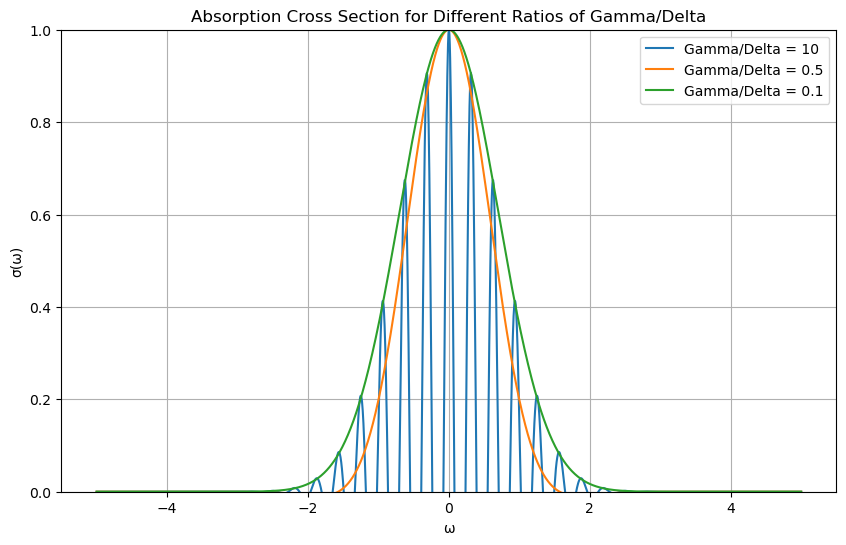
\includegraphics[max width=\textwidth]{acs.png}
  \caption{Absorption Cross Section for Different Line Shapes}
  \label{fig:acs}
\end{figure}
\section{Pump-probe and time resolved fluorescence}

Pump-probe and time resolved fluorescence measurement techniques both give the population of the excited state verse time. This allows for the population decay time to be determined, but separating dephasing is difficult.
\subsection{}
Draw the evolution of the Bloch sphere for an excitation pulse with area $3 \pi / 4$ for each of the three damping cases used in Problem 1 (only $T_{1}$, mixed $T_{1}$ and $T_{2}^{*}$, only $T_{2}^{*}$ ).
\subsubsection{Answer}
The initial excitation pulse of area \(3\pi/4\) is a pulse that tilts the Bloch vector away from the north pole by $\theta = 3\pi/4$, as shown in the drawing \ref{fig:bloch}.
\begin{figure}
    \centering
    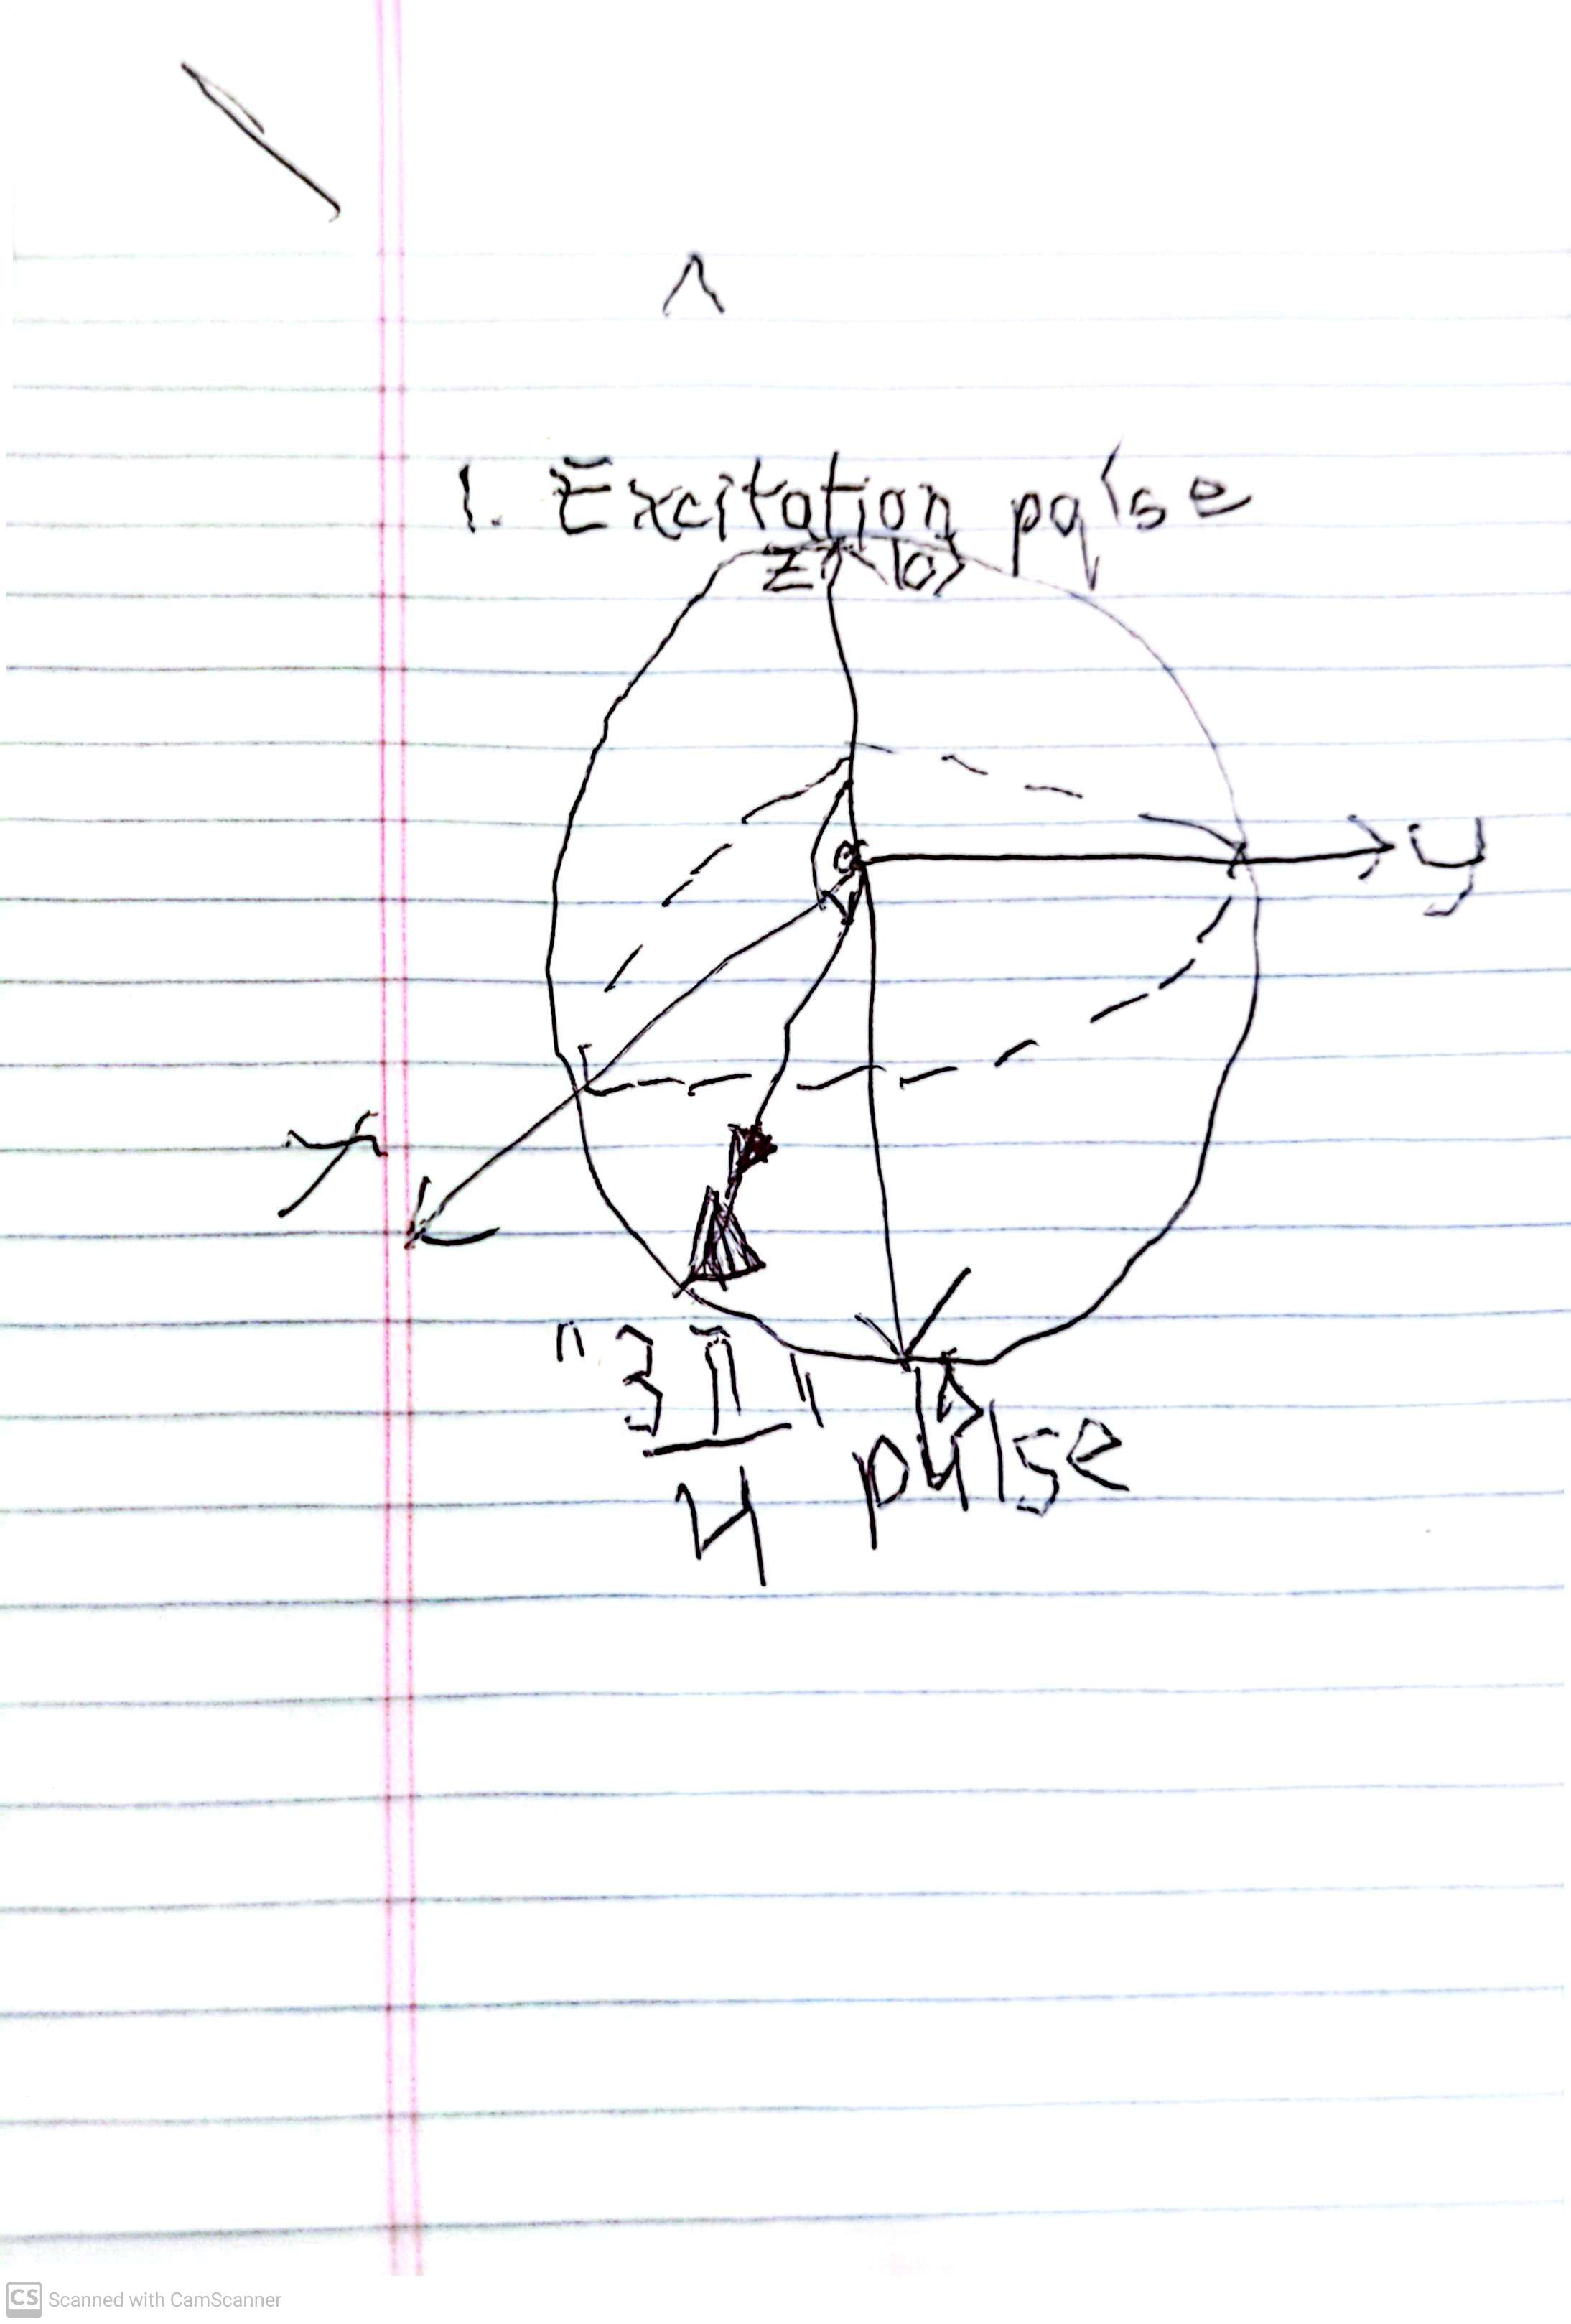
\includegraphics[width=\textwidth]{CamScanner 05-19-2024 21.01.jpg}
\caption{Bloch Sphere Evolution for Excitation Pulse of Area \(3\pi/4\)}
\label{fig:bloch}
\end{figure}
\textbf{Case 1: Only \(T_1\) (Longitudinal Relaxation)}

1. After the pulse, the Bloch vector is tilted away from the north pole.
2. Over time, the \(z\)-component relaxes back towards the north pole (ground state of $M_z$)



\textbf{Case 2: Mixed \(T_1\) and \(T_2^*\) (Both Relaxation and Dephasing)}

1. After the pulse, the Bloch vector is tilted away from the north pole.
2. Over time, the \(z\)-component relaxes back towards the north pole due to \(T_1\).
3. Simultaneously, the \(x\)- and \(y\)-components decay towards the origin due to \(T_2^*\) dephasing.
4. The Bloch vector's trajectory is a spiral that tightens towards the north pole and origin.



\textbf{Case 3: Only \(T_2^*\) (Dephasing)}

1. After the pulse, the Bloch vector is tilted away from the north pole.
2. The \(z\)-component remains unchanged since there is no \(T_1\) relaxation.
3. The \(x\)- and \(y\)-components decay towards the origin (ground state of $M_x$ and $M_y$) due to \(T_2^*\) dephasing.
\subsection{}
Plot the resulting excited state decay in each of the three damping cases on one plot. The measured signal is proportional to the intensity of the response function, or

$$
I_{\text {signal }} \sim|<\mu(t) \mu(0)>|^{2}
$$

from the Bloch diagrams. No work needed, just think.
\subsubsection{Answer}
As can be seen, the $T_2^*$ relaxation time is usually much shorter than the $T_1$ relaxation time. This can be seen from the fact that we are dealing with a $e^{-t^2}$ decay for the $T_2^*$ case, which is much faster than the $e^{-t}$ decay for the $T_1$ case. The mixed case is a combination of the two, so gives the best of both worlds. This is shown in the figure \ref{fig:decay}.
\begin{figure}
    \centering
    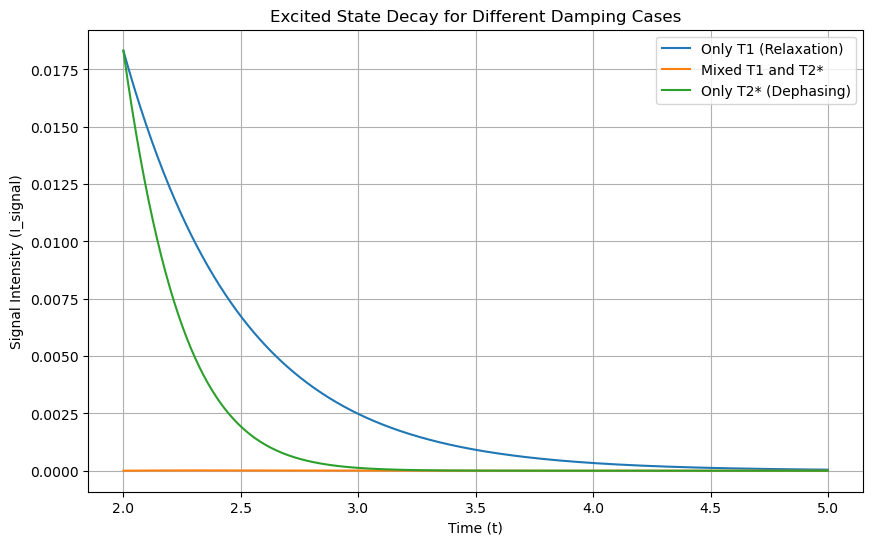
\includegraphics[max width=\textwidth]{output.png}
\caption{Excited State Decay for Different Damping Cases}
\label{fig:decay}
\end{figure}
% Inline Python code in the document
\begin{lstlisting}[language=Python]
import numpy as np
import matplotlib.pyplot as plt

# Time array
t = np.linspace(2, 5, 500)  # Start from 0 for full range

# Parameters for the cases
Gamma = 1.0
Delta = 1.0

# Signal intensities
I_T1n = np.exp(-2 * Gamma * t)
I_T2star = np.exp(-Delta**2 * t**2)

# I_T1_T2star will be a convolution of the two
I_T1_T2star = np.convolve(I_T1n, I_T2star, mode='full')[:len(t)] / len(t) # Normalize

# Plotting
plt.figure(figsize=(10, 6))
plt.plot(t, I_T1n, label='Only T1 (Relaxation)')
plt.plot(t, I_T1_T2star, label='Mixed T1 and T2*')
plt.plot(t, I_T2star, label='Only T2* (Dephasing)')
plt.xlabel('Time (t)')
plt.ylabel('Signal Intensity (I_signal)')
plt.title('Excited State Decay for Different Damping Cases')
plt.legend()
plt.grid(True)
plt.show()
\end{lstlisting}
\newpage
\section{}
In Problems 1 and 2, we have seen that homogenous and inhomogenous broadening is very hard to separate, although these factors determine the measured signal. If we measure the photon echo, however, we can separate these effects. The pulse train to create a photon echo is
shown in the following diagram:

\begin{center}
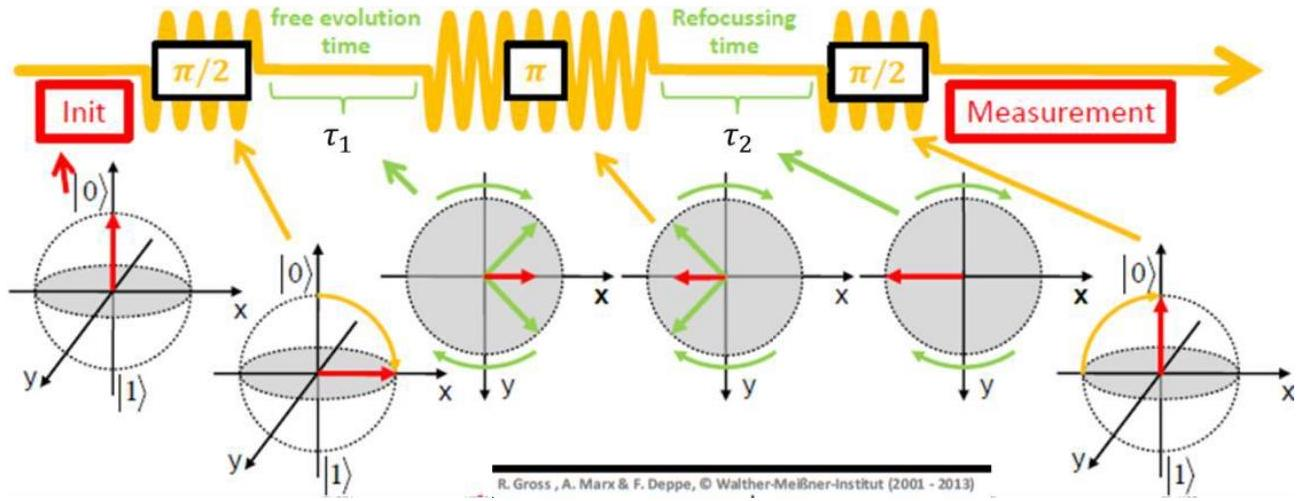
\includegraphics[max width=\textwidth]{2024_05_19_b95480aad91fe1b645d5g-2}
\end{center}
\subsection{}
Plot the photon echo for the three damping constants of Problem 1 and Problem 2. The polarization for the above pulse ordered diagram can be roughly modeled as:


$$
\left|P\left(\tau_{1}, \tau_{2}\right)\right| \sim\left|R^{(3)}\right| \sim\left|\exp \left(j \omega_{0}\left(\tau_{1}-\tau_{2}\right)-\Gamma\left(\tau_{1}+\tau_{2}\right)-\frac{\Delta^{2}\left(\tau_{1}-\tau_{2}\right)^{2}}{2}\right)\right|
$$

Plot the polarization against $\tau_{2}$, taking $\tau_{1}=5, \omega_{0}=1, \Gamma=\frac{1}{2}$-and varying $\Delta=0.05,1,5$ for the three cases. Please plot all three curves on the same graph, do not normalize the heights.

You should notice the interplay between homogenous and inhomogenous broadening in the photon echo. Make sure you understand the position and shape of the photon echo based on including inhomogenous and homogenous broadening in the above Bloch diagrams. No work is needed, just think about it.
\subsubsection{Answer}
The value of $\Delta =5$ corresponds to the lowest value of $\frac{\Gamma }{\Delta }$, so in the green curve in \ref{fig:echo}, we are looking at the Gaussian curve. The center of its peak along the horizontal time axis of $\tau_2$ is the greatest of the three because there has been a lot of inhomogeneity in the transverse orientation of the spins and so it will take the largest amount of time for refocusing.
\begin{figure}
  \centering
  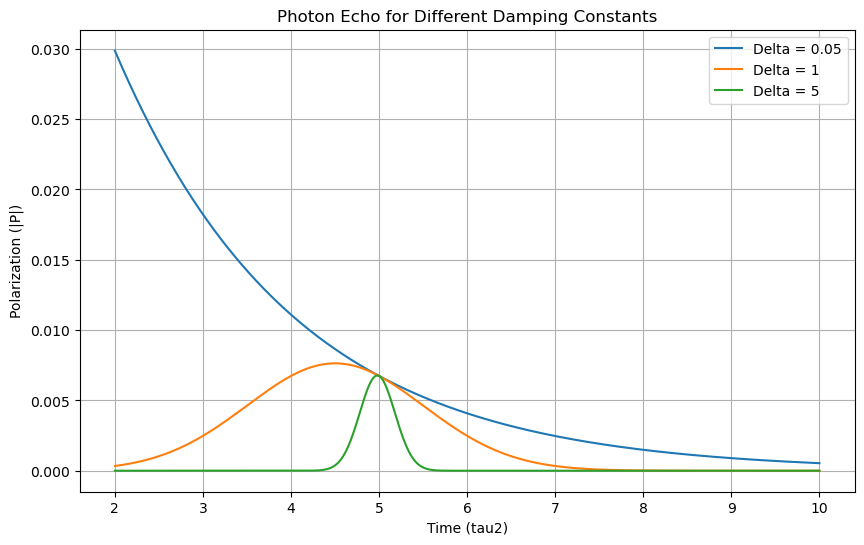
\includegraphics[max width=\textwidth]{p3a.png}
  \caption{Photon Echo for Different Broadening Mechanisms}
  \label{fig:echo}
\end{figure}
\subsection{}

We can use the photon echo to separate the two broadening mechanisms. To demonstrate this, plot the photon echo against $\tau_{2}$ for several values of $\tau_{1}$. Do this for the case when the inhomogenous broadening is much larger than the homogenous ( $\Gamma=\frac{1}{2}$ and $\Delta=5$ ). Please plot all curves on the same graph, do not normalize the heights. Add a line giving the maximum value of the photon echo for all $\tau_{1}=\tau_{2}$. The result should be exponential.

\subsubsection{Answer}
This plot is shown in \ref{fig:echo2}. We see a resemblance of an exponential decay for the line connecting the $\tau_{1}=\tau_{2}$ points. If a finer grid of points for $\tau_{1}$ were used, then this curve would be smoother. We can also notice that when the value of tau one is smaller, that means the spins have had less time to dephase, so tau 2 can be lower because the time needed for refocusing is smaller. A trend that can also be commented on is that the curve for smaller values of $\tau_1 = \tau_2$ is higher than the curve for larger values of $\tau_1 = \tau_2$. This is because the spins have had less time to dephase, so the echo is stronger.\\
\begin{figure}
  \centering
  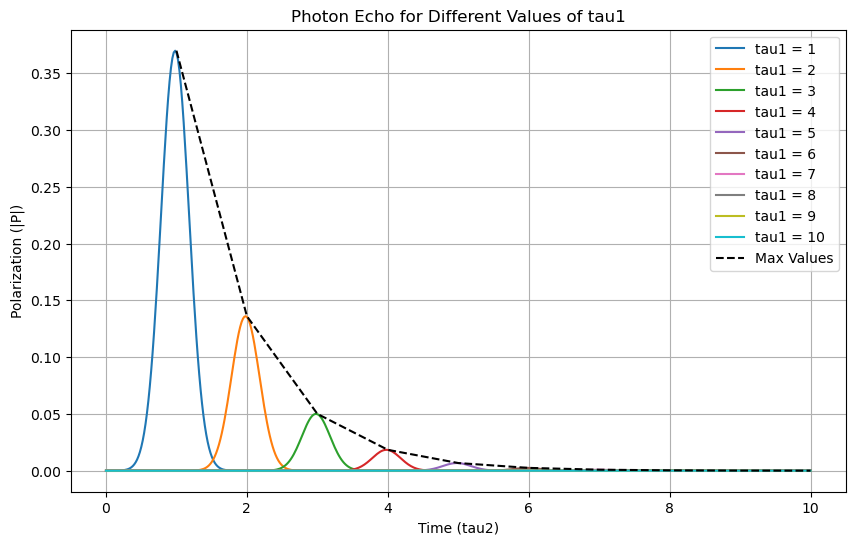
\includegraphics[max width=\textwidth]{echo2.png}
  \caption{Photon Echo for Different $\tau_{1}$}
  \label{fig:echo2}
\end{figure}

The inhomogenous broadening will be rephased at a time of $2 \cdot \tau_{1}$ from the initial pulse creating a photon echo with a strength independent of the value of $\tau_{1}$. The strength of the photon echo will therefore only be determined by the extent of inhomogenous decay at 2 . $\tau_{1}$, since this cannot be reversed. Therefore, by looking at the strength of the photon echo versus $\tau_{1}$, the homogenous lifetime could be determined.

Note: The above model and response function is based on a two beam photon echo. Experimentally, three pulses are usually used and the inhomogenous and homogenous broadening are extracted a little differently from what is presented, although the use of rephasing is still the key.


\end{document}